\begin{apendicesenv}

\partapendices

\chapter{Termo de Abertura do Projeto}

\subsection{Descrição do projeto}

O projeto é uma plataforma de ciclismo interativa com imersão em ambiente de realidade virtual e monitoramento de dados fisiológicos e de desempenho. O usuário utilizará uma bicicleta acoplada ao sistema e um óculos de realidade virtual, interagindo com um ambiente virtual gamificado emulado pelo Oculus por meio da bicicleta, pedalando e utilizando o guidão. 

\subsection{Justificativa do projeto}

Treinos de ciclismo em ambientes fechados é uma demanda relevante para profissionais e entusiastas do esporte. Diversas soluções para esse ponto existem, incluindo circuitos \textit{indoor} e bicicletas fixas de exercício que simulam parte da estrutura de uma bicicleta tradicional. Tais soluções são o padrão atual do mercado, mas possuem algumas limitações. Uma delas é o fato de que bicicletas de exercício não possuem uma sensação similar o suficiente a uma bicicleta comum, além de possuírem indicadores limitados a quantidade aproximada de calorias gastas e outros. Treinamento em circuitos \textit{indoor} requerem deslocamento do usuário ao local.

Um sistema de ciclismo interativo permitiria uma experiência de ciclismo verossímil e gamificada, servindo de estímulo de treinamento aos usuários, tanto pela qualidade da experiência quanto pela praticidade de uso.


\subsection{Objetivos do projeto}

Como proposta de solução, o projeto a ser desenvolvido tem como objetivo emular a sensação de andar de bicicleta de uma forma verossímil, utilizando uma bicicleta tradicional como base e a realidade virtual para emular diferentes ambientes de ciclismo, a fim de aproximar a experiência do usuário no sistema à experiência real, à medida em que dados do seu desempenho são coletados. O projeto também procura ser de fácil acesso e utilização, utilizando-se de diretrizes de usabilidade para isso. Com isso, busca-se uma maior utilização do sistema no dia-a-dia, para que o  usuário tenha seu desempenho medido de forma constante.

\subsection{Requisitos de alto nível}

O projeto terá uma bicicleta acoplada a uma plataforma, um óculos de realidade virtual e um \textit{notebook} para a execução do \textit{software}. O sistema também contará com um sistema que permite a elevação da bicicleta e aumento no esforço necessário para movimentar o pedal, simulando subidas e decidas.

O jogo contará com dois circuitos, um com pista lisa e duas curvas inspirado em pistas tradicionais e um com caminho com elevações e diversas curvas, inspirado em ambientes abertos. Cada usuário poderá ter uma conta local, em que serão registrados preferências e dados de desempenho. Os dados de desempenho devem ser apresentados em forma de gráficos para o usuário e acessíveis a partir do menu principal. A bicicleta deverá ser projetada de tal forma que caso o usuário venha a perder o equilibrio este não caia da plataforma. Além disso, deverá haver aproveitamento de parte da energia produzida pelo usuário ao pedalar.
 
\subsection{Subsistemas Identificados}

Foram identificados quatro subsistemas no projeto: o subsistema eletrônico, responsável pela construção dos componentes eletrônicos, captação e interpretação dos sinais da bicicleta e do usuário, o subsistema de energia, responsável pela geração de energia elétrica a partir da energia mecânica obtida pelos movimentos de pedalada do usuário, o subsistema de estrutura, responsável pela construção da plataforma e adaptação da bicicleta e componentes do Oculus na montagem do projeto, e o subsistema de software, responsável pela interface de interação com o usuário e apresentação do cenário virtual.

\subsection{Riscos}

Os principais riscos que podem ocorrer durante o projeto são os referentes a inexperiência da equipe na utilização das ferramentas necessárias para construção da plataforma, bem como nas tecnologias a serem utilizadas no desenvolvimento. Outros riscos que podem ocorrer e que afetam diretamente ao projeto, são os riscos relacionados a utilização de equipamentos de alto custo e do espaço cedido para equipe no LART. Outro risco de grande impacto é a integração no último mês do projeto de todos os módulos a serem desenvolvidos.

\subsection{Resumo do cronograma de marcos}

O desenvolvimento da solução terá três marcos principais, caracterizados como pontos de controle. A primeira fase do projeto é a fase de planejamento e tem duração de três semanas e será finalizada no dia do primeiro ponto de controle, entre seis a nove de setembro. A segunda fase é a fase de construção dos subsistemas e inicia dia primeiro de setembro e termina dia três de novembro, com uma duração de, aproximadamente, dois meses. O segundo ponto de controle ocorre entre os dias primeiro e três de novembro. A terceira fase é a de integração dos subsistemas, inicia dia três de novembro e termina dia primeiro de dezembro. O terceiro ponto de controle ocorre entre três a seis de dezembro.

\subsection{Resumo do orçamento}

O custo total do projeto será de R\$ 8.995,34, deste valor total, R\$ 7.317,64, refere-se aos custos do óculos \textit{Rift} e o Desktop do LART que a equipe já possui.

\begin{table}[htp]
\centering
\caption{Orçamento}
\label{orcamento}
\begin{tabular}{|l|l|}
\hline
Simulador de Ambiente Virtual & R\$ 7.317,64 \\ \hline
Sistema de Alimentação de Energia & R\$ 383,99 \\ \hline
Estrutura & R\$ 900,00 \\ \hline
Sistemas de aquisição e controle & R\$ 393,71 \\ \hline
\multicolumn{2}{|c|}{\textbf{R\$ 8.995,34}} \\ \hline
\end{tabular}
\end{table}

\subsection{Lista das partes interessadas}

Dentre os interessados, estão os patrocinadores e alunos de graduação de engenharia da Universidade de Brasília campus Gama que cursam a disciplina de Projeto Integrador em Engenharia 2.

\subsection{Requisitos para a aprovação do projeto}

O projeto deverá ser aprovado por seus patrocinadores e professores da disciplina de Projeto Integrador em Engenha2.

\subsection{Gerência do projeto}

O projeto será gerenciado por Matheus Pereira Santana, graduando em Engenharia Eletrônica, sendo ele o gerente geral. Mas terá também outros quatro estudantes responsavéis por gerenciar cada subsistema da Plataforma de Ciclismo Interativa.

\subsection{Patrocinadores}

O projeto contará com dois patrocinadores, a professora Carla Rocha e o professor Augusto Brasil, que possuem interesse no produto a ser gerado ao final do semestre. 

\chapter{Modelo de Negócio}

\begin{center}
    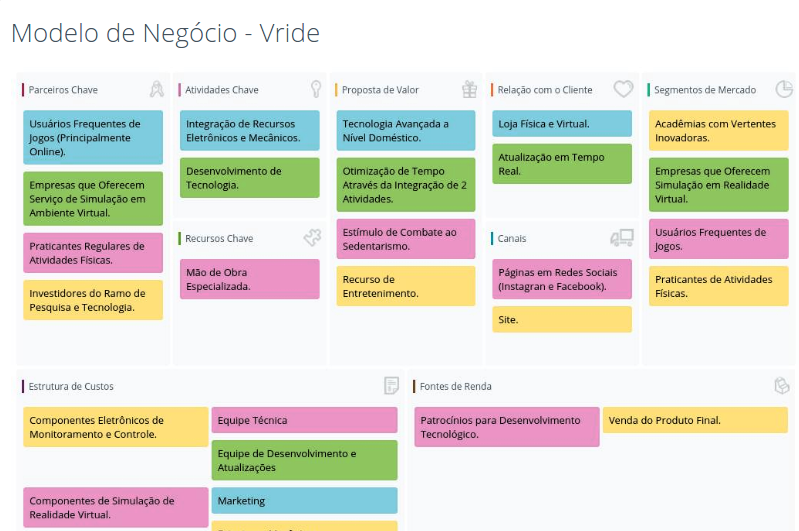
\includegraphics[scale=0.5]{figuras/canvas}
       \captionof{figure}{ Modelo Canvas de Negócio. }
       \label{canvas}
   \end{center}  

\section{Plano de Marketing}


\subsection{SUMÁRIO EXECUTIVO}
 
\subsubsection{Descrição do Produto ou Serviço }
 \textit{Ramo de atividade:}
Empresa responsável pela fabricação  de um produto voltado ao entretenimento aliado a prática de atividade física. 
 \textit{Mercado de atuação:}Mercado de equipamentos esportivos; mercado de entretenimento; mercado de tecnologia. 
 \textit{Segmento de mercado:} Praticantes de atividades físicas, com especial interesse pelo ciclismo e/ou consumidores de jogos e simulações em realidade virtual. 

\subsection{ANÁLISE DO AMBIENTE}

\subsubsection{Definição do Ambiente Externo} 

Nossos concorrentes são variados: Produtos que oferecem exclusivamente recursos para a prática de atividade física, jogos diversos, ambientes de simulação virtual tais como os de shopping que oferecem jogos diversos como montanha russa e cenários de ficção científica, etc. 
A inserção no mercado é dificultada por ser um produto de segmento exclusivo (que alia dois segmentos muito destoantes, jogos e atividade física), então o público – alvo acaba se tornando restrito. Além da necessidade de mão de obra especializada para a produção do produto final, mesmo quando feito em escala, o que encarece bastante o preço final. 

\subsubsection{Público Alvo}

\begin{itemize}
\item 
O produto pode ser comprado por usuários que buscam ter em suas casas um equipamento de prática de atividade física.
\item
O produto pode ser comprado por amantes de jogos que querem vencer o sedentarismo. 
\item
O produto pode ser comprado por acadêmias que desejam inovar em seus equipamentos. 
\item
O produto pode ser comprado por lojas de fliperamas / playgrounds.

\item
O produto pode ser comprado por lojas de shopping que já oferecem outros jogos ambientes de realidade virtual.
\end{itemize}

 
\subsection{PESQUISA DE MERCADO}
 
\subsubsection{Problema de pesquisa}

Identificar, a partir de dados como idade, sexo e remuneração mensal familiar, o público – alvo específico deste produto, assim como sua propessão e interesse em adquirir o mesmo.
 
\subsubsection{Objetivos da pesquisa}

\begin{itemize}
\item 
Identificar qual a idade média dos possíveis usuários do produto; 
\item
Identificar qual o sexo do usuário e se tal informação influencia na escolha do uso ou não do produto; 
\item
Identificar a renda mensal familiar do possível usuário e se isso influencia ou não na compra do produto; 
\item
Identificar quantos dos possíveis usuários já praticam atividade física; 

\item
Identificar quantos dos possíveis usuários já usam constantemente jogos.
\end{itemize}


\subsubsection{Fontes de dados}

Os dados foram obtidos a partir de um formulário criado no portal do Google Formulários e foi divulgado por meio de redes sociais em grupos de praticantes de ciclismo e de comunidades de trocas de informações de jogos online. 
 
\subsubsection{Amostra}
O formulário foi respondido por um total de 42 participantes. 
 
\subsubsection{Instrumento de pesquisa}
 Formulário do Google Doc. 

\subsubsection{Análise dos dados}
 
\subsubsubsection{Idade}

O objetivo da pergunta é identificar a idade média do possível utilizador do equipamento e utilizar esta informação para realizar um perfil do usuário. 

\begin{center}
    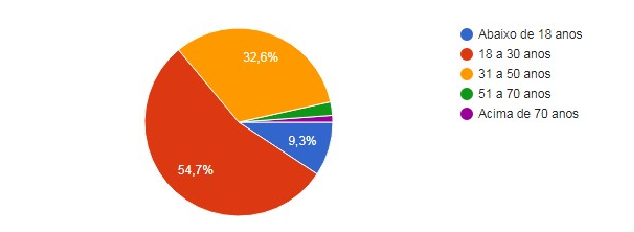
\includegraphics[scale=0.7]{figuras/idade}
       \captionof{figure}{ Idade dos possíveis usuários. Fonte: Dados da Pesquisa  }
       \label{idade}
   \end{center}  
 
Percebe-se que 54,7\% dos participantes da pesquisa possuem a idade entre 18 e 30 anos, sendo assim considera-se que grande parte dos possíveis usuários pode ser de idade jovem. 

Observou-se também que a quantidade de pessoas na faixa de 31 a 50 anos também é grande, o que indica que os consumidores também são adultos, indicando assim que o produto pode despertar interesse em diversos tipos de pessoas e não só como o esperado, que a população jovem (mais familiarizada com as tecnologias como a do jogo), levando a conclusão que o produto desperta o interesse nas mais variadas faixas etárias 
 
\subsubsubsection{Sexo}

O objetivo da pergunta foi mais uma vez identificar o perfil do possível usuário sabendo o sexo do mesmo. 
\begin{center}
    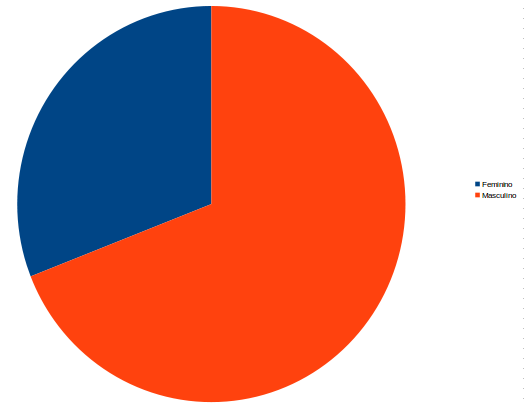
\includegraphics[scale=0.7]{figuras/sexo}
       \captionof{figure}{ Sexo dos possíveis usuários. Fonte: Dados da Pesquisa  }
       \label{sexo}
   \end{center}  
 
Percebe-se pela pesquisa que a maior parte dos participantes é do sexo masculino, uma observação pertinente acerca disto é que este resultado não expressa que mais homens se interesse pelo produto, porém no grupo amostral a quantidade de homens era significantemente maior que a de mulheres. 

\subsubsubsection{Renda Familiar Mensal}

Procura-se analisar por meio desta pergunta a correlação entre a renda familiar mensal e o possível interesse do cliente, afim de avaliar se as pessoas que tem interesse no produto possivelmente teriam possibilidade financeira de comprar ou se este seria um impencílio.

\begin{center}
    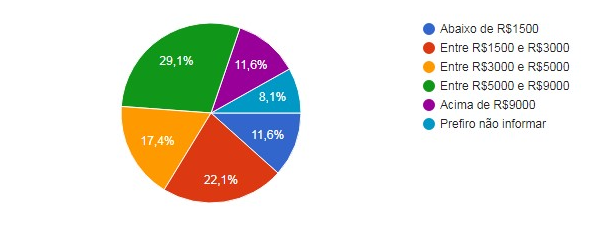
\includegraphics[scale=0.7]{figuras/renda}
       \captionof{figure}{ Renda Média dos possíveis usuários. Fonte: Dados da Pesquisa  }
       \label{renda}
   \end{center}  
 
Percebeu-se que a renda familiar dos participantes se encontra de forma bem variada, mas cabe ressaltar a presença de 29,1\% dos participantes entre as rendas familiares mensais de R$5000 e R$9000, uma vez que este valor se asemelha mais ao valor previsto para o custo do produto final. 
 
\subsubsubsection{Você é usuário frequente de jogos ?}

Com esta pergunta procurou-se saber quantos dos entrevistados são usuários frequentes de jogos.
\begin{center}
    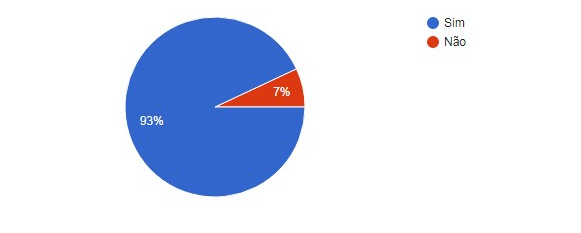
\includegraphics[scale=0.7]{figuras/jogos}
       \captionof{figure}{ Usuários frequentes de jogos. Fonte: Dados da Pesquisa}
       \label{jogos}
 \end{center}   

Percebe-se que a grande parte dos entrevistados relatam em seu cotidiano buscar e utilizar jogos, o que é algo muito positivo para contribuir com que estas pessoas possam vir a adquirir o produto. 
 
\subsubsubsection{Você pratica atividades físicas regularmente ?}
Procurou-se por meio desta analisar se os possíveis clientes já estão engajados em alguma outra forma de prática de exercício físico. 
                                           \begin{center}
    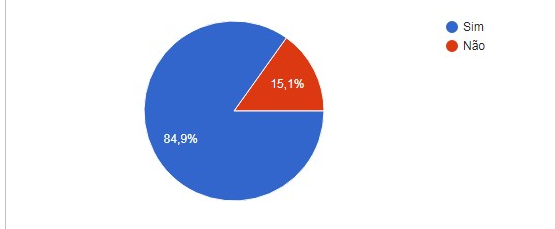
\includegraphics[scale=0.7]{figuras/atividadefisica}
       \captionof{figure}{ Praticantes de Atividades Físicas. Fonte: Dados da Pesquisa}
       \label{atividadefisica}
 \end{center}   
 
Percebe-se que a grande parte dos entrevistados relatam já praticarem atividades físicas, o que contribui positivamente para serem possíveis clientes, uma ve que praticantes sempre buscam novas modalidades para ter um estímulo extra. 

\subsubsubsection{Qual o seu nível de interesse em um jogo com realidade virtual integrado a uma bicicleta, onde é possível simultaneamente jogar e praticar atividade física ?}

Com esta pergunta tem-se o objetivo de analisar o interesse dos entrevistados  no produto. 
 
 \begin{center}
    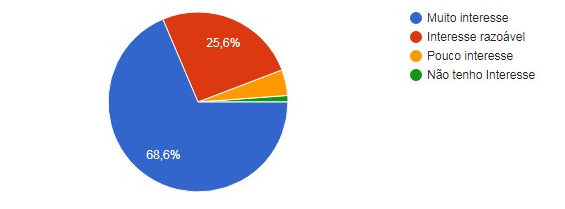
\includegraphics[scale=0.7]{figuras/interesse}
       \captionof{figure}{ Interesse dos usuários no produto. Fonte: Dados da Pesquisa}
       \label{interesse}
 \end{center}   
Percebe-se que grande parte dos entrevistados, 94,2\%, possui algum interesse pelo produto, sendo que desses, 68,6\% possuem muito interesse em utilizar o produto, o que valida o público – alvo escolhido. 


\subsection{POSICIONAMENTO DE MERCADO} 

\subsubsection{ Diferencial Competitivo}

Diferentemente dos equipamentos já existentes, o produto não apenas promove a prática de atividade física ou o lazer por meio dos jogos, mas simultaneamente oferece dois serviçoes de interesse, o que torna o produto bem mais atraente pois além de realizar a atividade que usualmente o usuário já praticava ou tem interesse vai ter o bônus de estar se divertindo com um jogo ou aproveitando o tempo de lazer para se exercitar.
Atualmente, não há nenhum produto equivalente sendo vendido no Brasil. 

\subsubsection{Público alvo}
O público-alvo do produto são pessoas praticantes de atividades físicas e/ou usuários de jogos.
\subsubsection{Marca}
\subsubsubsection{O nome do negócio e produto/serviço} 
O nome ‘Vride’ é claro e objetivo, evidenciando nosso principal propósito e a principal finalidade do produto: ciclismo integrado ao ambiente de realidade virtual.
\subsubsubsection{Logotipo}
O símbolo, assim como o nome, representa o principal objetivo do aplicativo: Promover a prática do ciclismo, para tanto o logotivo elucida isto através da figura da bicicleta, o nome rift também presente na logo tem por objetivo remeter o usuário a o conceito de realidade virtual.

A cor vermelha simboliza a confiança, e está fortemente associada com energia e vitalidade. Vermelho em algumas culturas é também a cor que representa a inteligência e o progresso tecnológico, o que vai de encontro a associar uma tecnologia recente (realidade virtual) com uma tecnologia mais antiga, a bicicleta. 

 
\includegraphics[scale=0.7]{figuras/logo}
       \captionof{figure}{ Logotipo Vride}
       \label{interesse}
 \end{center}   

\subsection{ESTRATÉGIA DE MARKETING}
\subsubsection{Produto}
	O Vride consiste em um jogo de realidade virtual que é integrado a uma bicicleta, o que proporcionará ao usuário utilizar os dois recursos simultaneamente, o jogo e um equipamento de atividade física. 
\subsubsection{Promoção}
 	A divulgação será realizada por meio de uma página no Facebook que inicialmente será propagada em comunidades que sabe-se serem usuárias de produtos e/ou atividades similares a proposta, tais como grupos de ciclismo, grupos de estilo de vida saudável, grupos de inovações tecnologia, grupos de “fãs” de jogos de realidade aumentada , entre outros. Esta estratégia será monitorada com base no feedback dos comentários dos potenciais usuários na própria publicação nos grupos, pelo aumento na quantidade de curtidas da página, assim como pelo aumento da quantidade de contatos para possível compra do produto. Esta estratégia terá duração de 1 mês e será utilizada apenas para a propagação inicial do produto e para validar a aceitação do mesmo dentro do público-alvo estipulado, posteriormente serão adotados anúncios pagos no próprio facebook. 
	 Após 2 meses da implementação dos anúncios pagos (e 3 da divulgação inicial do produto) serão avaliados os resultados obtidos para decidir pela continuidade ou não deste tipo de divulgação além de possivelmente traçar estratégias de divulgação mais precisas, tais como divulgação de anúncios em sites de vendas já consolidados no mercado.
 	
\subsubsection{Controle e Avaliação}

 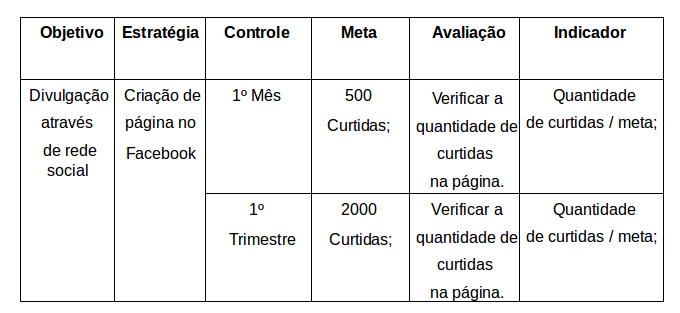
\includegraphics[scale=0.6]{figuras/tabelaa}
       \captionof{figure}{Controle e Avaliação}
       \label{controle}
 \end{center}  

\chapter{Esquemáticos}
\input{anexos/esquematicos}

\chapter{Layout}
\input{anexos/layout}

\chapter{Códigos}

\chapter{Configuração de Rede}

O Raspberry foi programado para atuar como duas interfaces principais. Como access point da rede wireless e como broker do protocolo MQTT. As configurações utilizadas para tal função foram:

\begin{enumerate}
    \item Atualização e instalação dos pacotes:
        \begin{itemize}
            \item \$ sudo apt-get update
            \item \$ sudo apt-get install isc-dhcp-server
            \item \$ sudo apt-get install hostapd
            \item \$ sudo apt-get install mosquitto
            \item \$ sudo apt-get install mosquitto-dev
        \end{itemize}

    \item No arquivo \textit{/etc/dhcp/dhcp.conf} fazer as seguintes alterações:
        \begin{itemize}
            \item Comentar com \# as linhas:
                option domain-name "example.org";

                option domain-name-servers

                ns1.example.org, ns2.example.org
            \item Descomentar as linhas:
                authoritative
            \item Escrever no fim do arquivo:

                subnet 10.0.0.0 netmask 255.255.255.0 $\{$

                \hspace*{6mm}    range 10.0.0.2 10.0.0.255;

                \hspace*{6mm}    option domain-name-servers 8.8.8.8;

                \hspace*{6mm}    option domain-name "local";

                \hspace*{6mm}    option routers 10.0.0.1;

                \hspace*{6mm}    option broadcast-address 10.0.0.255;

                \hspace*{6mm}    default-lease-time 600;

                \hspace*{6mm}    max-lease-time 7200;
                $\}$
        \end{itemize}
    \item No arquivo \textit{/etc/network/interfaces} colocar no arquivo:
        auto lo

        iface lo inet loopback

        iface eth0 inet dhcp

        allow-hotplug wlan0

        iface wlan0 inet static

            \hspace*{6mm} address 10.0.0.1

            \hspace*{6mm} netmask 255.255.255.0

	    \hspace*{6mm} gateway 10.0.0.1

    \item Criar o arquivo \textit{/etc/hostapd/hostapd.conf} com o seguinte texto:

        interface=wlan0

        driver=nl80211

        ssid=bikerift\_broker

        country\_code=US

        hw\_mode=g

        channel=6

        macaddr\_acl=0

        auth\_algs=1

        ignore\_broadcast\_ssid=0

        wpa=2

        wpa\_passphrase=bikerift

        wpa\_key\_mgmt=WPA-PSK

        wpa\_pairwise=CCMP

        wpa\_group\_rekey=86400

        ieee80211n=1

        wme\_enabled=1

    \item Alterar no arquivo \textit{/etc/default/hostapd} a linha \#DAEMON\_CONF

por DAEMON\_CONF="/etc/hostapd/hostapd.conf"

    \item No arquivo \textit{/etc/sysctl.conf} descomentar a linha: net.ipv4.ip\_forward=1.

    \item Executar no terminal:
        \begin{itemize}
            \item \$ sudo sh -c "echo 1 > /proc/sys/net/ipv4/ip\_forward"

            \item \$ sudo iptables -t nat -A POSTROUTING -o eth0 -j MASQUERADE

            \item \$ sudo iptables -A FORWARD -i eth0 -o wlan0 -m state --state RELATED,ESTABLISHED -j ACCEPT

            \item \$ sudo iptables -A FORWARD -i wlan0 -o eth0 -j ACCEPT

            \item \$ sudo sh -c "iptables-save > /etc/iptables/rules.v4"

            \item \$ sudo service hostapd start

            \item \$ sudo service isc-dhcp-server start

            \item \$ sudo update-rc.d hostapd enable

            \item \$ sudo update-rc.d isc-dhcp-server enable

        \end{itemize}
\end{enumerate}


\chapter{Desenhos Técnicos}
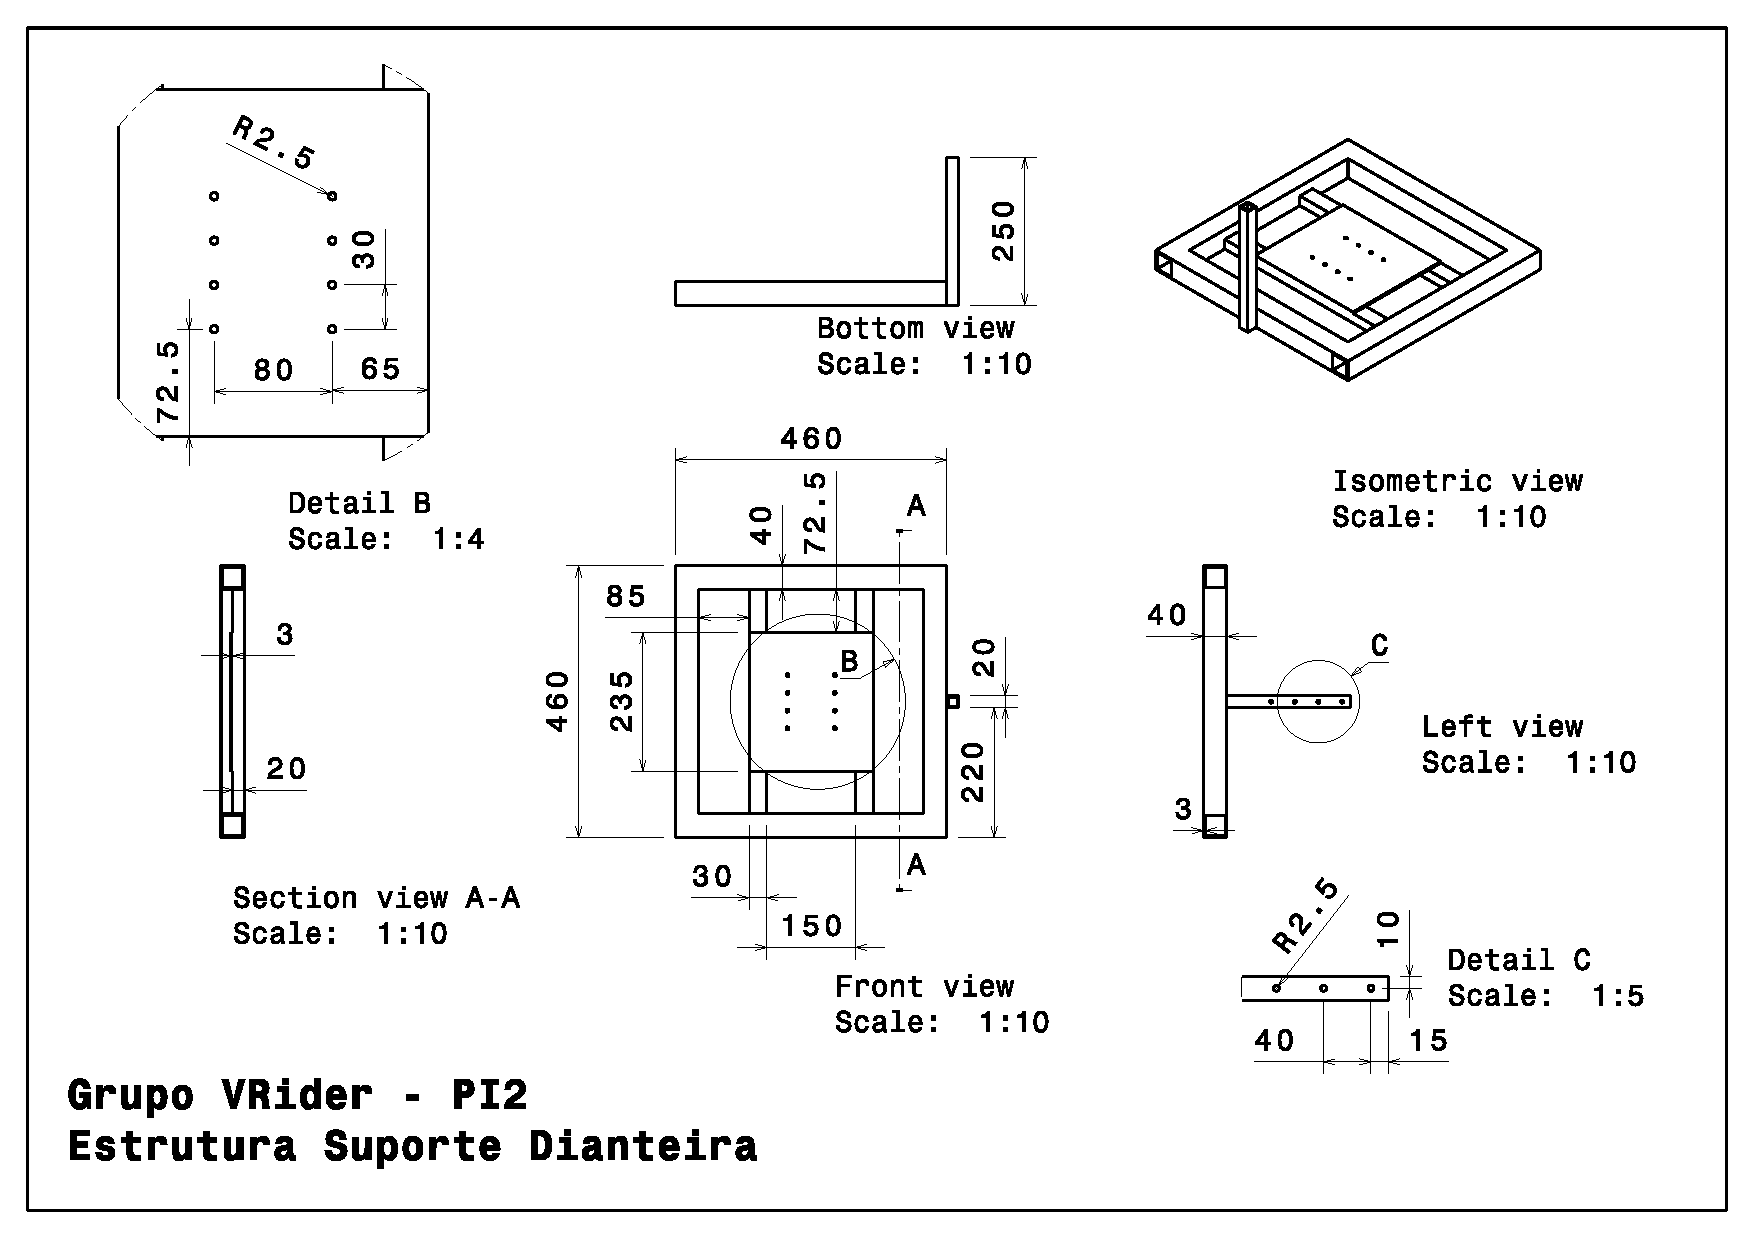
\includepdf[pages=1]{pdfs/dte_estrutura_suporte_dianteira.pdf} \label{anexo_base_frontal}
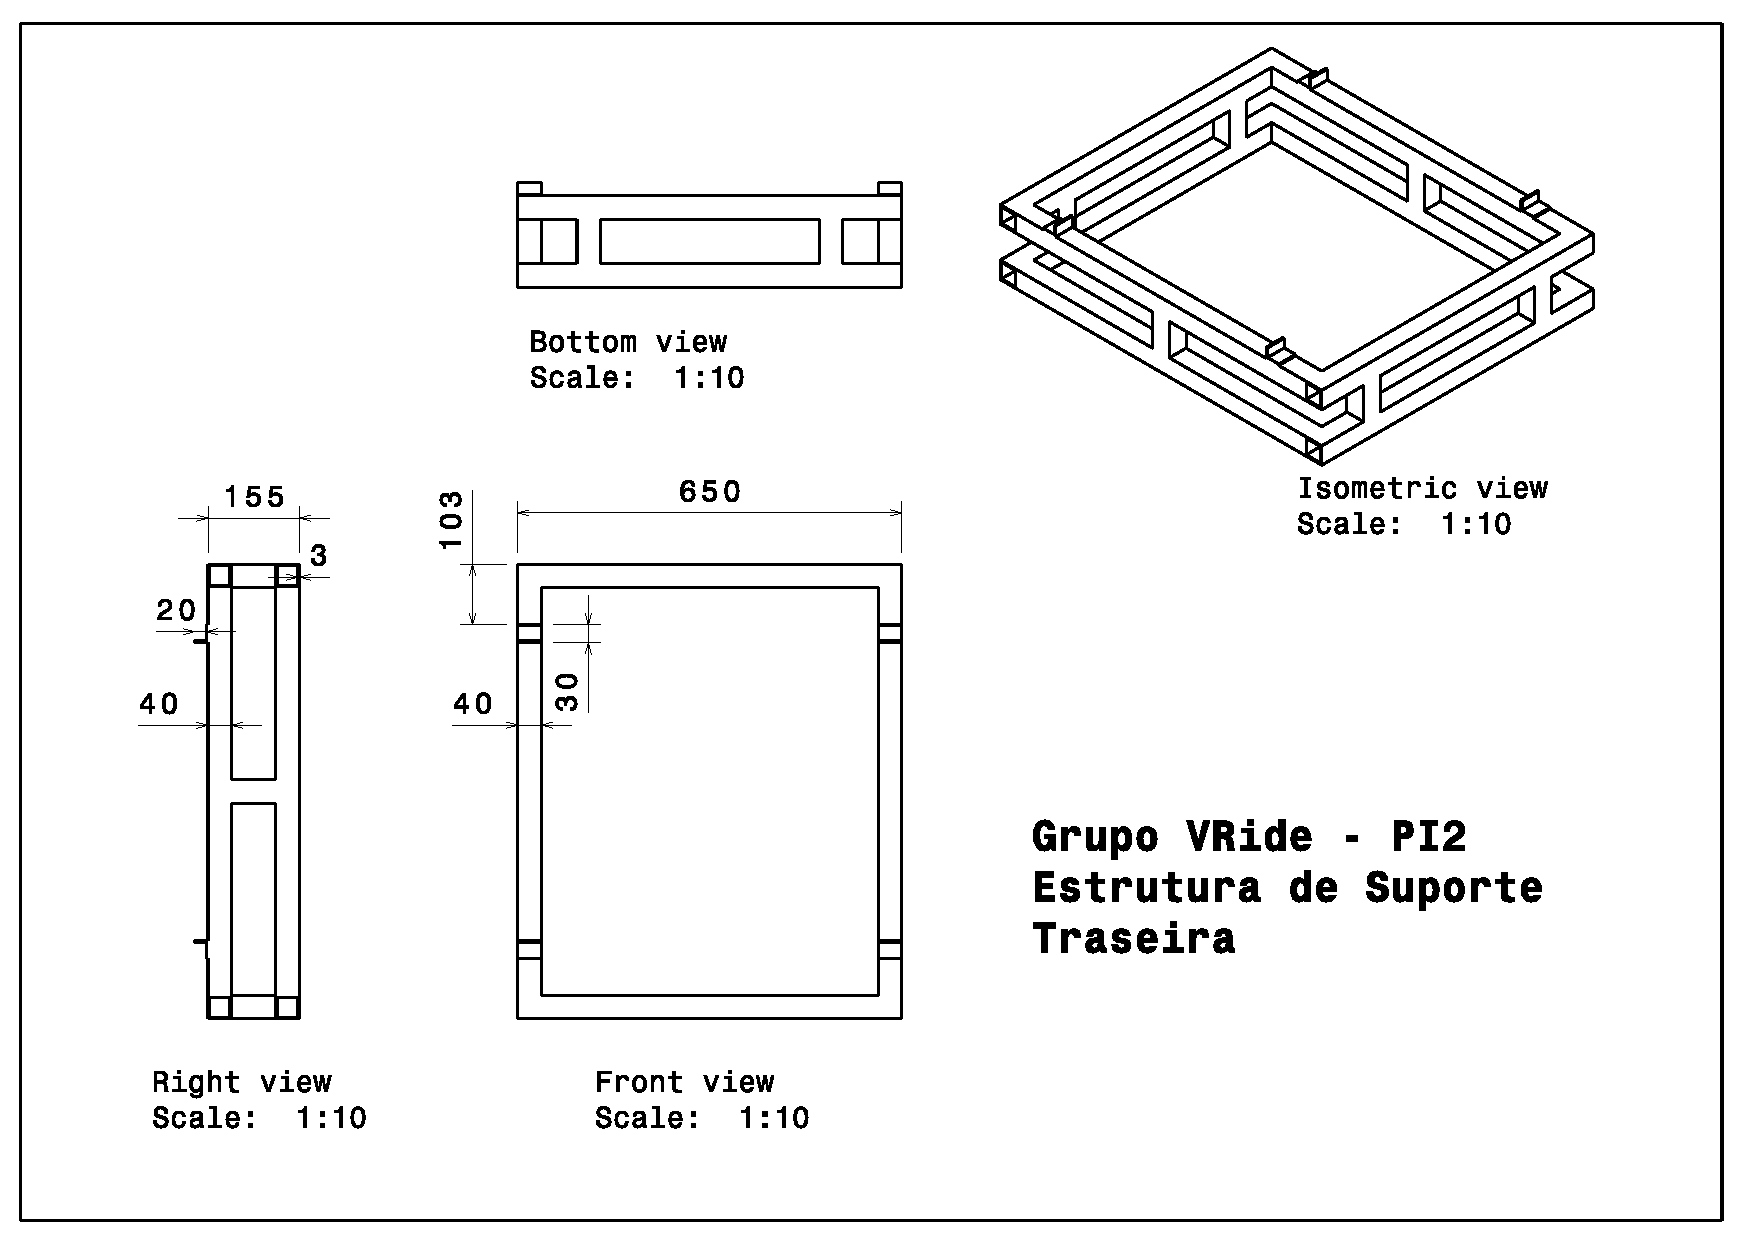
\includepdf[pages=1]{pdfs/dte_estrutura_suporte_traseira.pdf} \label{anexo_base_traseira}
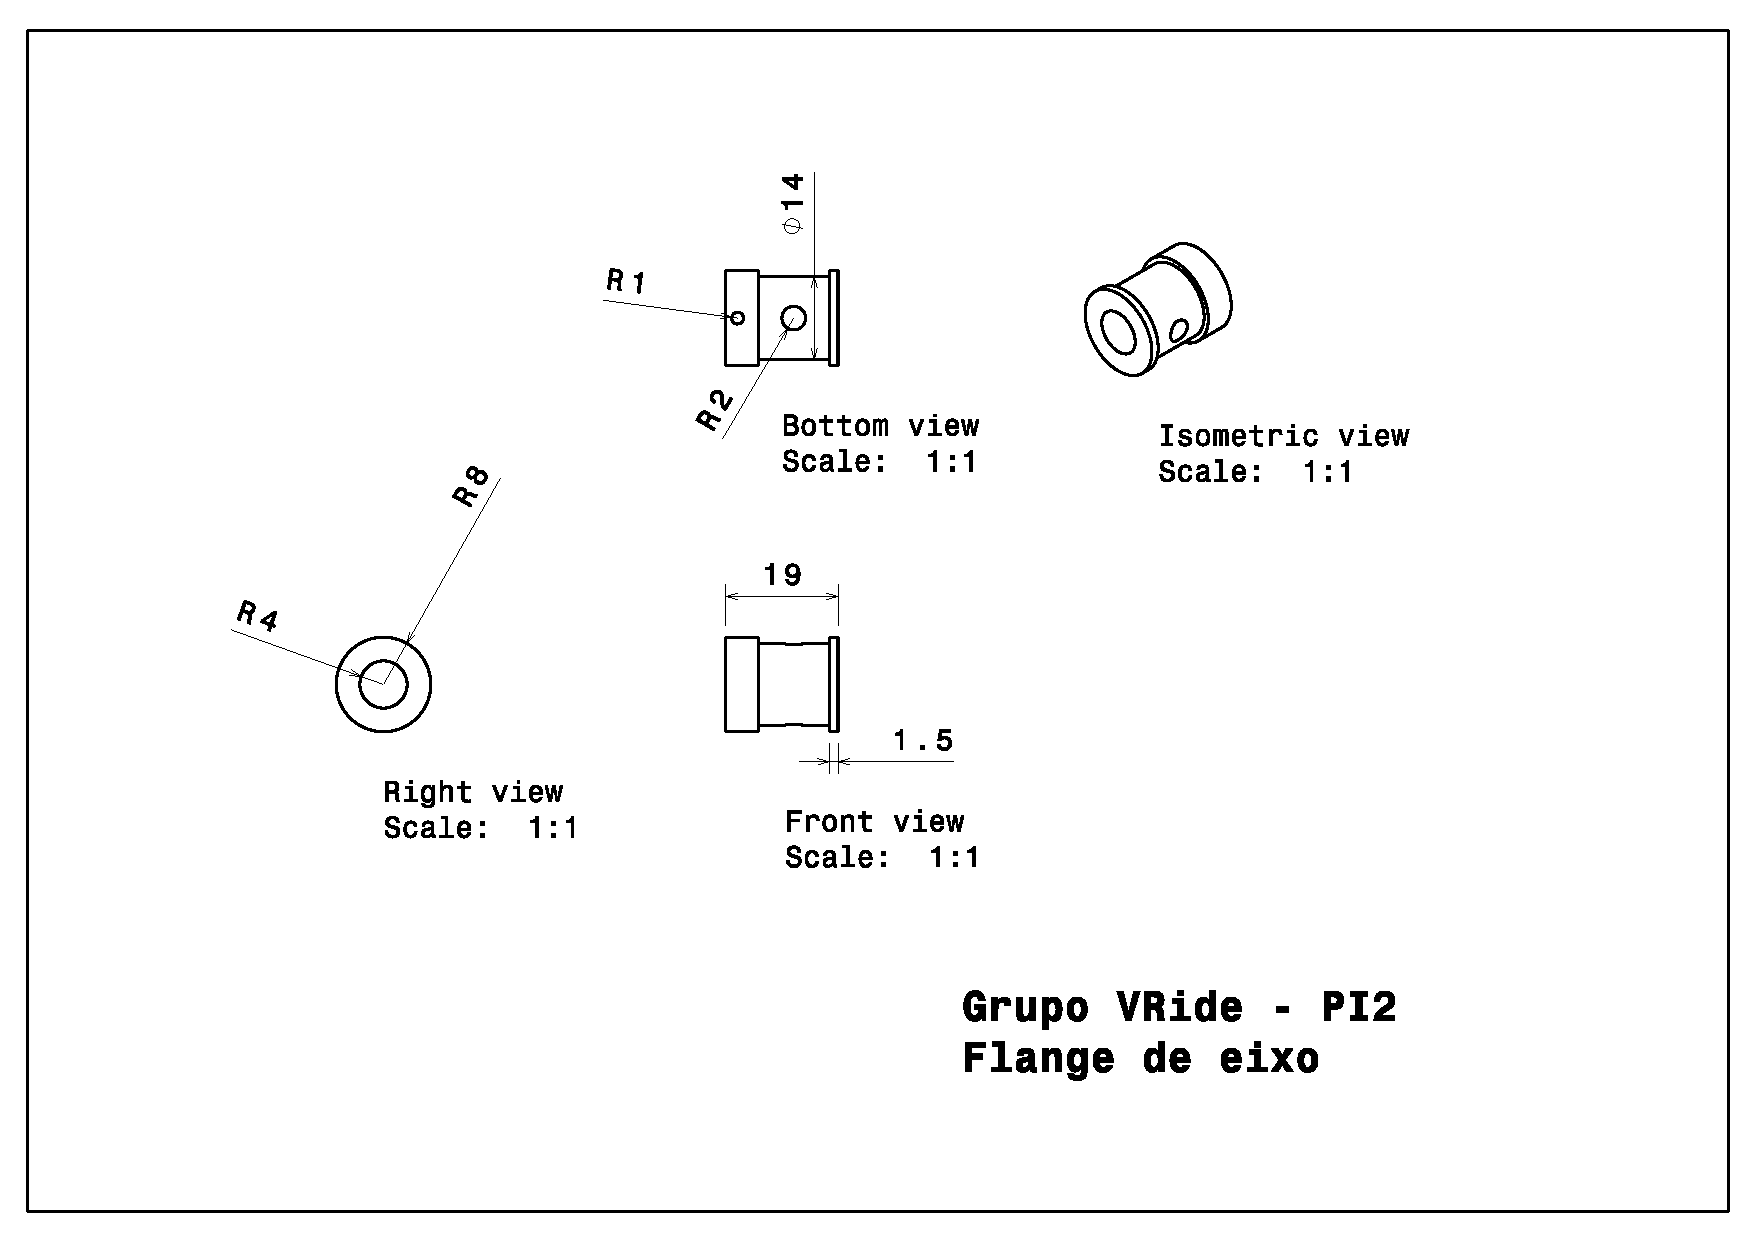
\includepdf[pages=1]{pdfs/dte_flange_eixo.pdf} \label{anexo_enrolador}
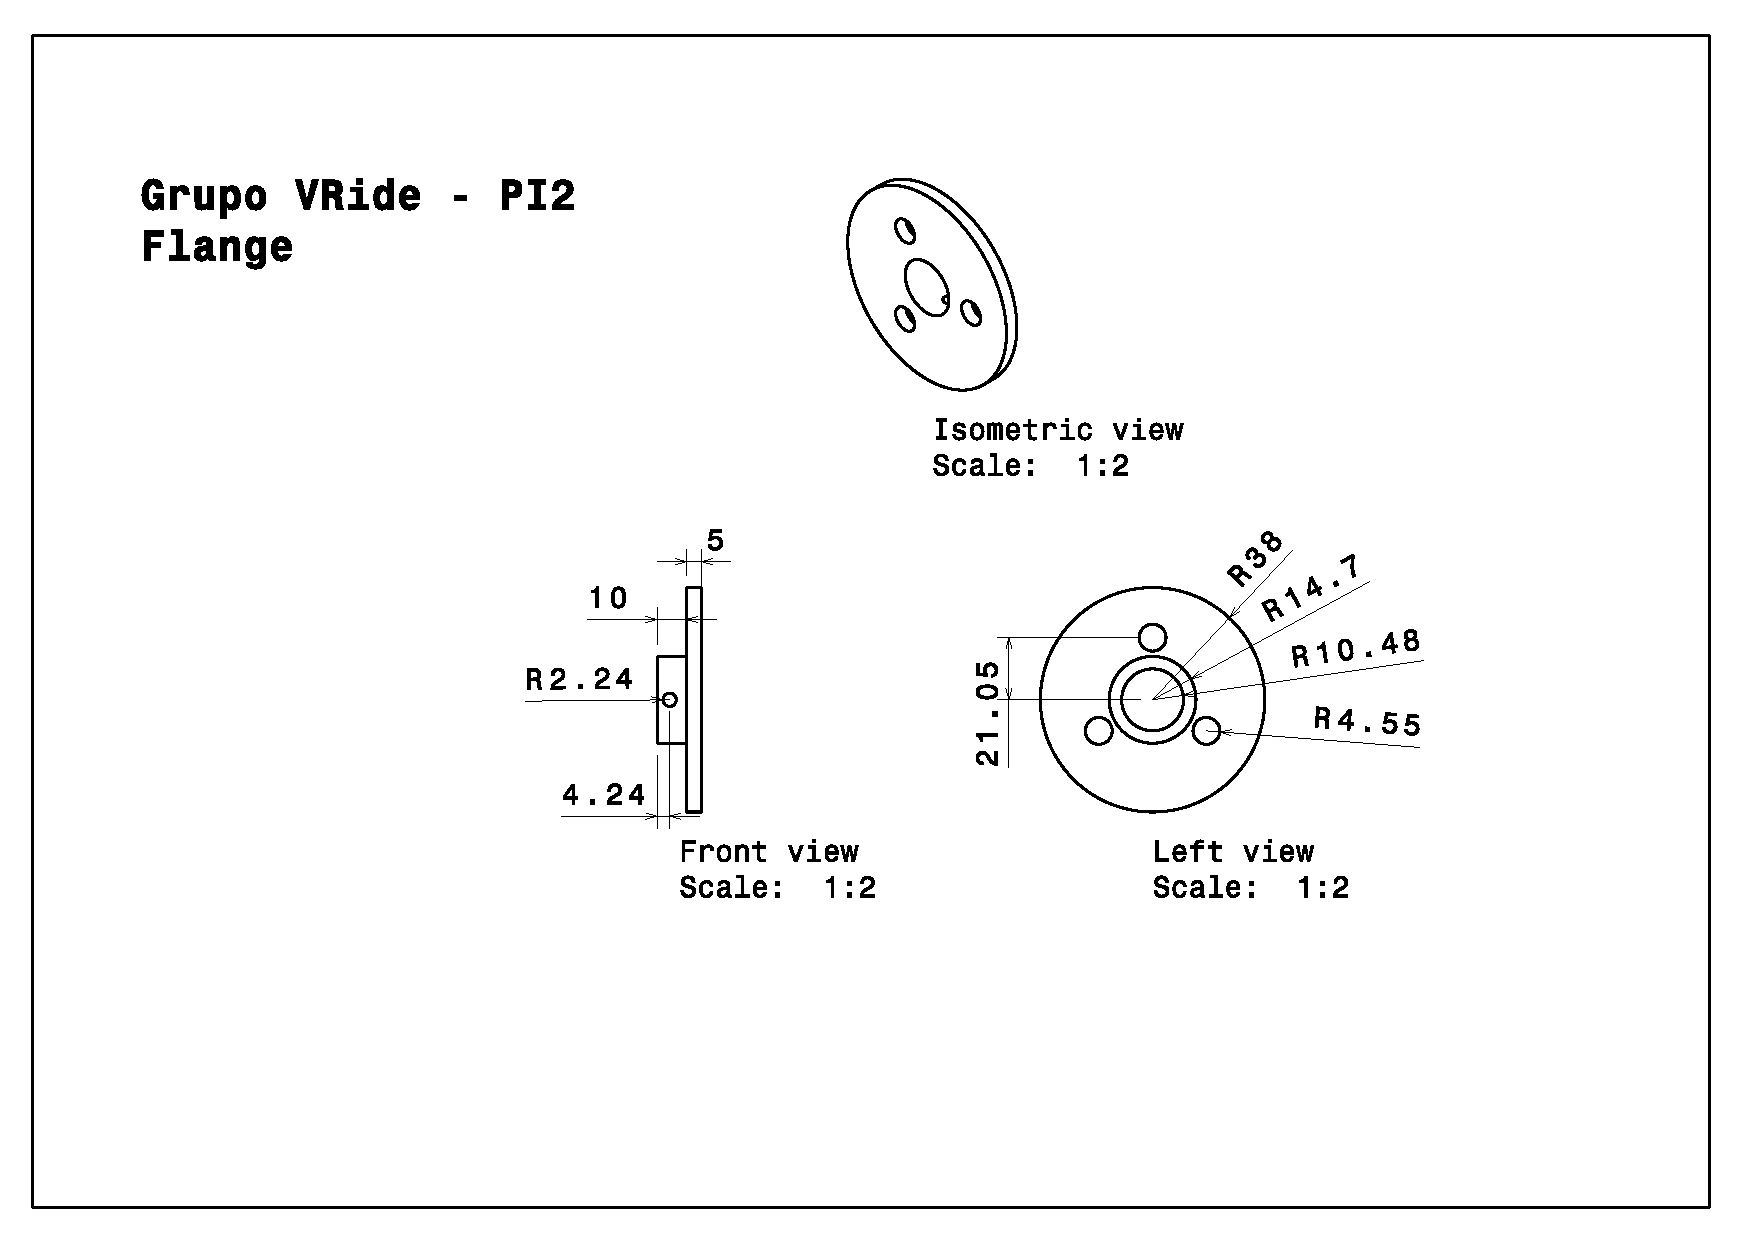
\includepdf[pages=1]{pdfs/dte_flange.pdf} \label{anexo_flange}
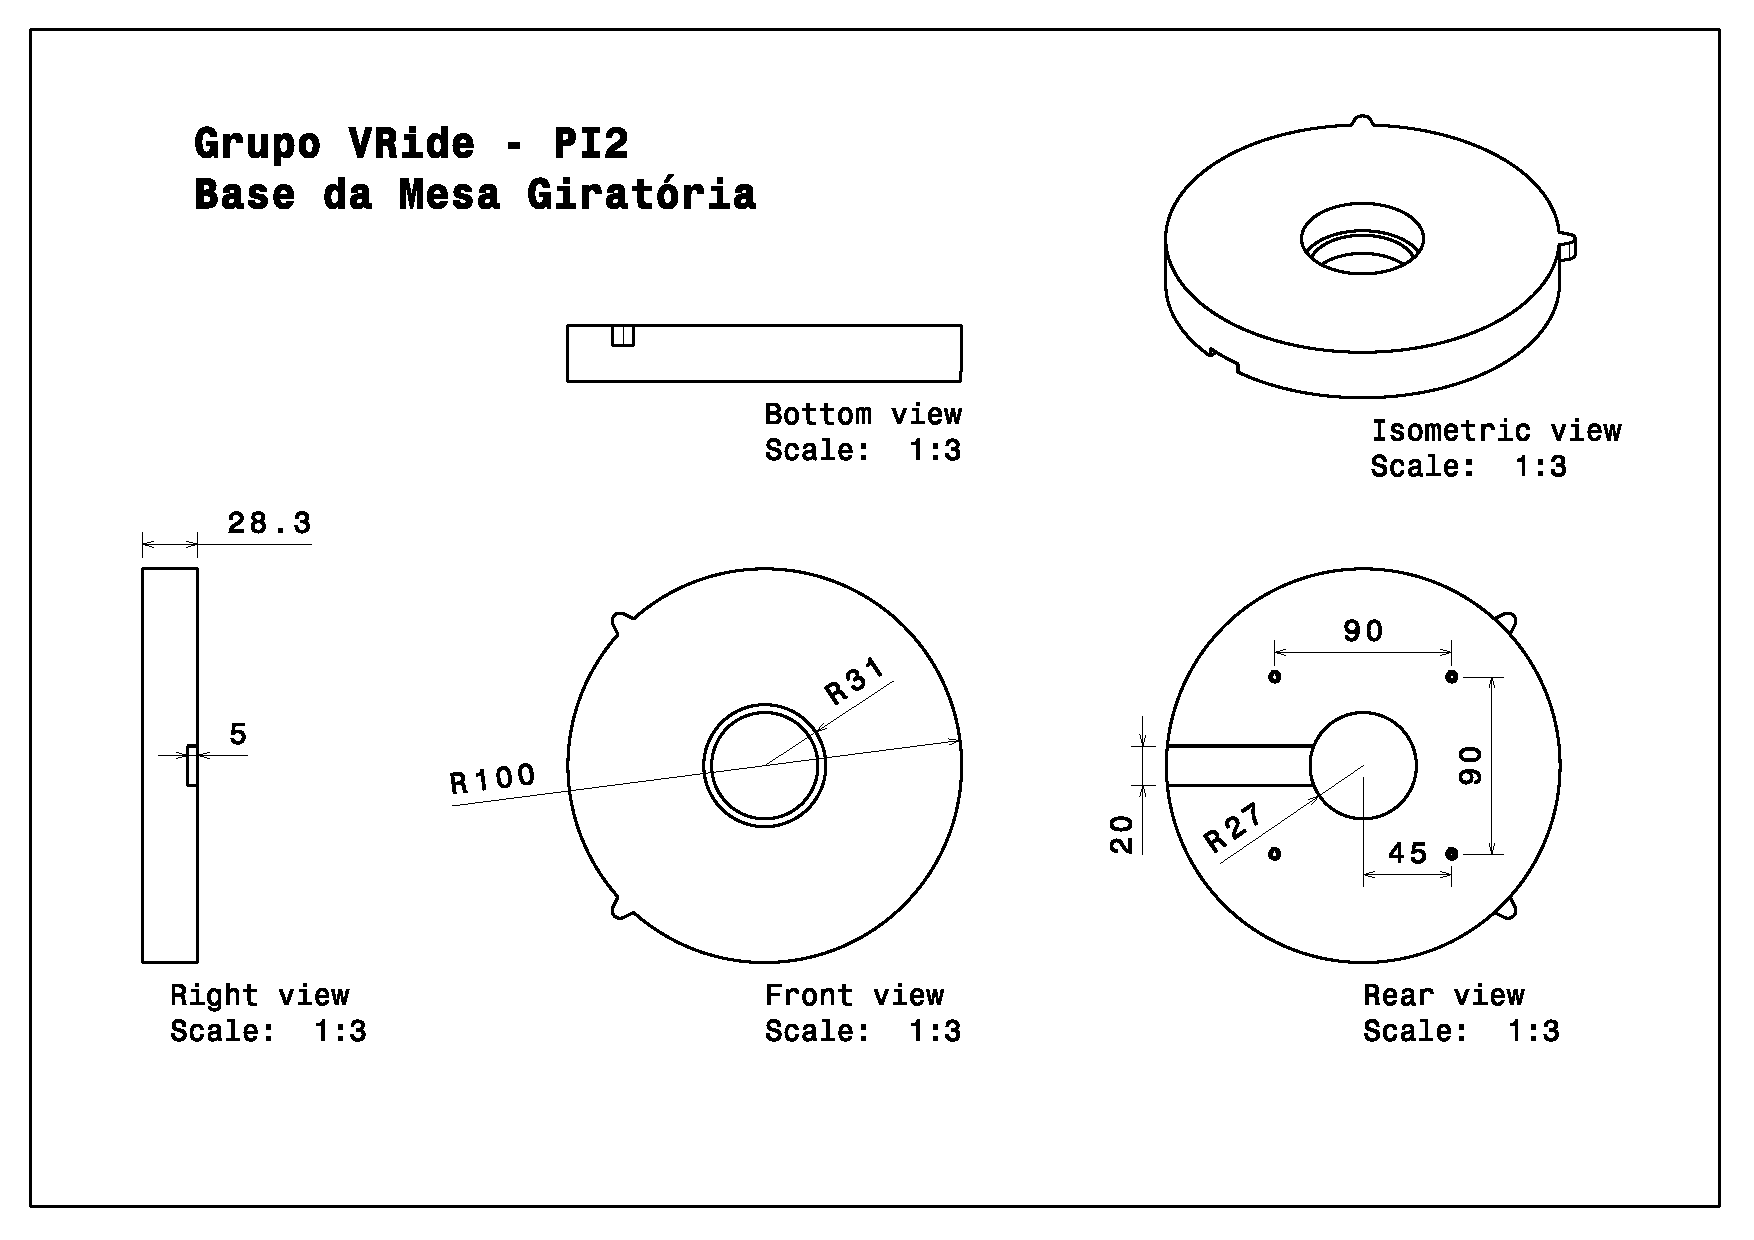
\includepdf[pages=1]{pdfs/dte_basemesagiratória.pdf} \label{anexo_megi_inferior}
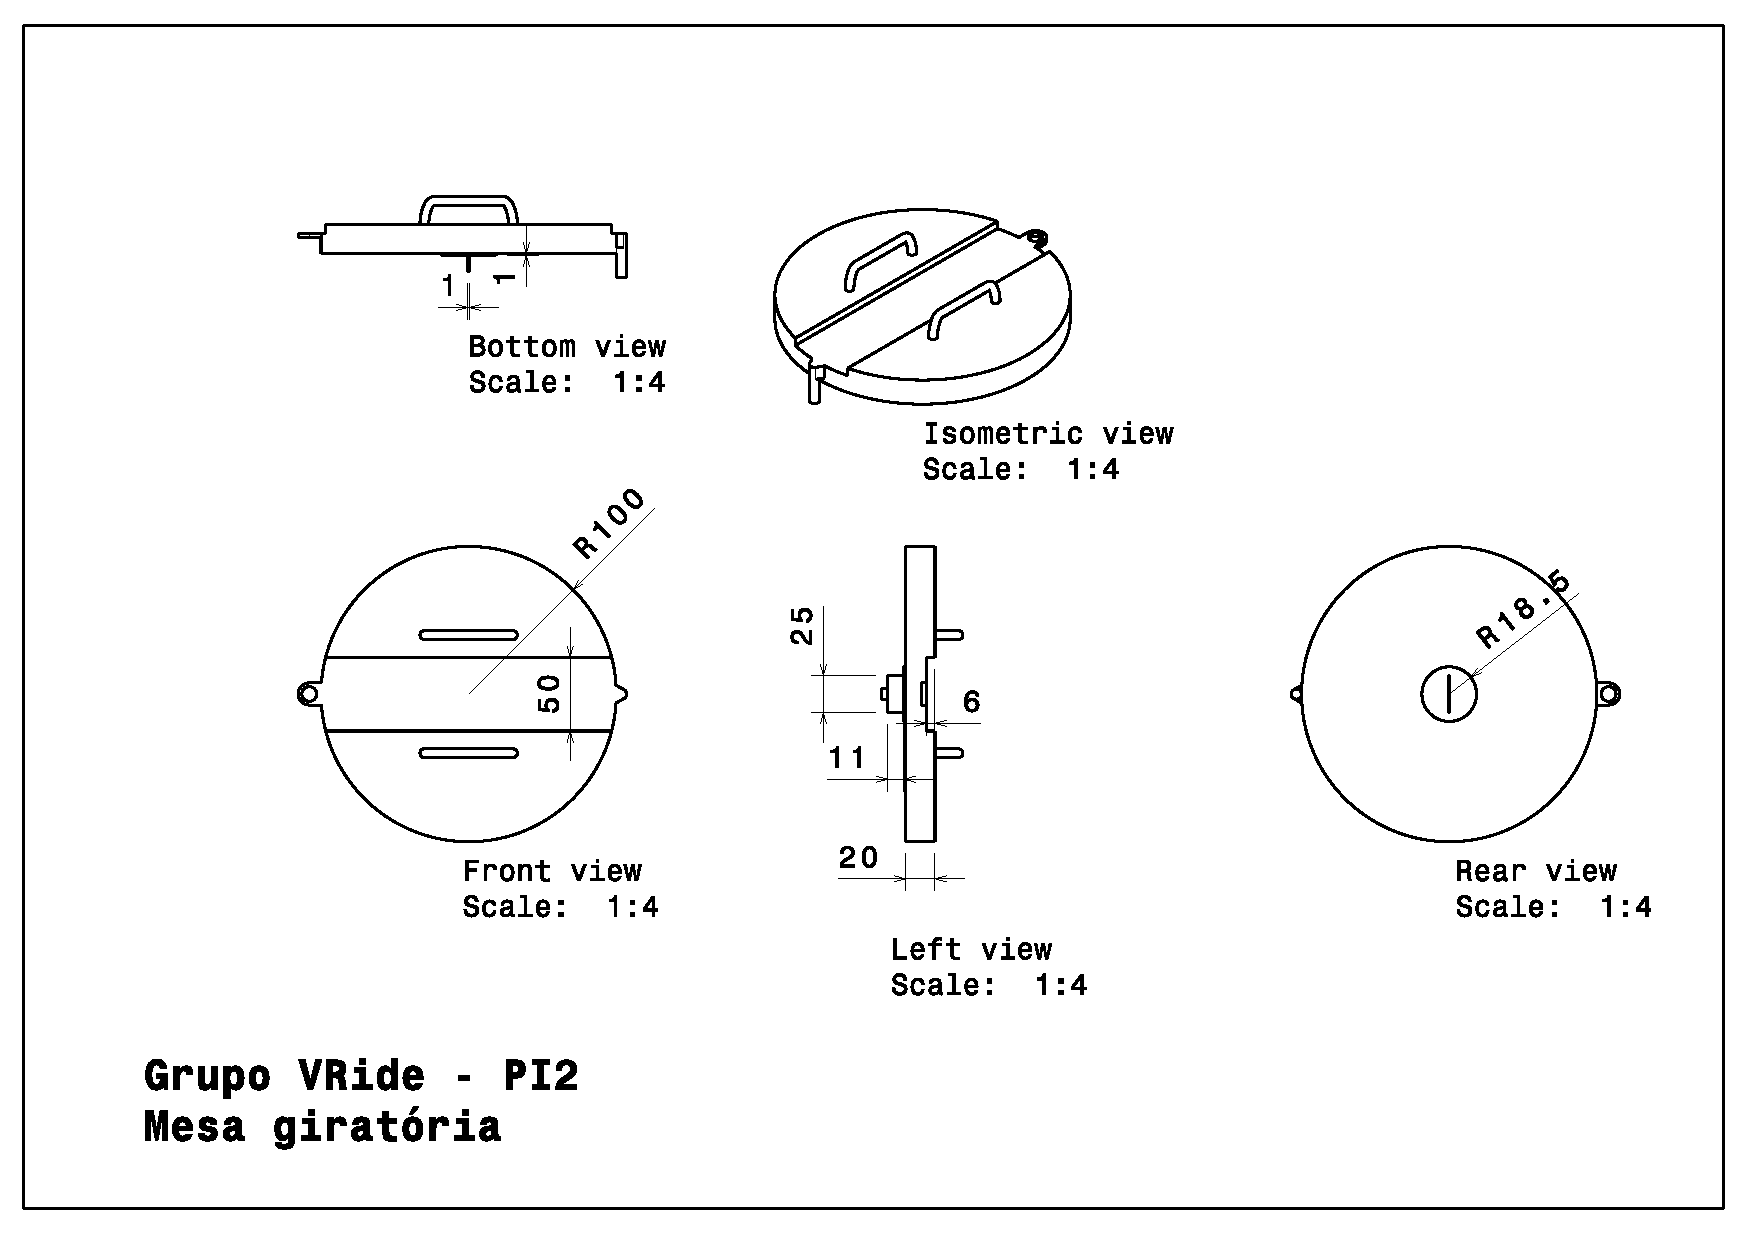
\includepdf[pages=1]{pdfs/dte_mesa_giratória.pdf} \label{anexo_megi_superior}
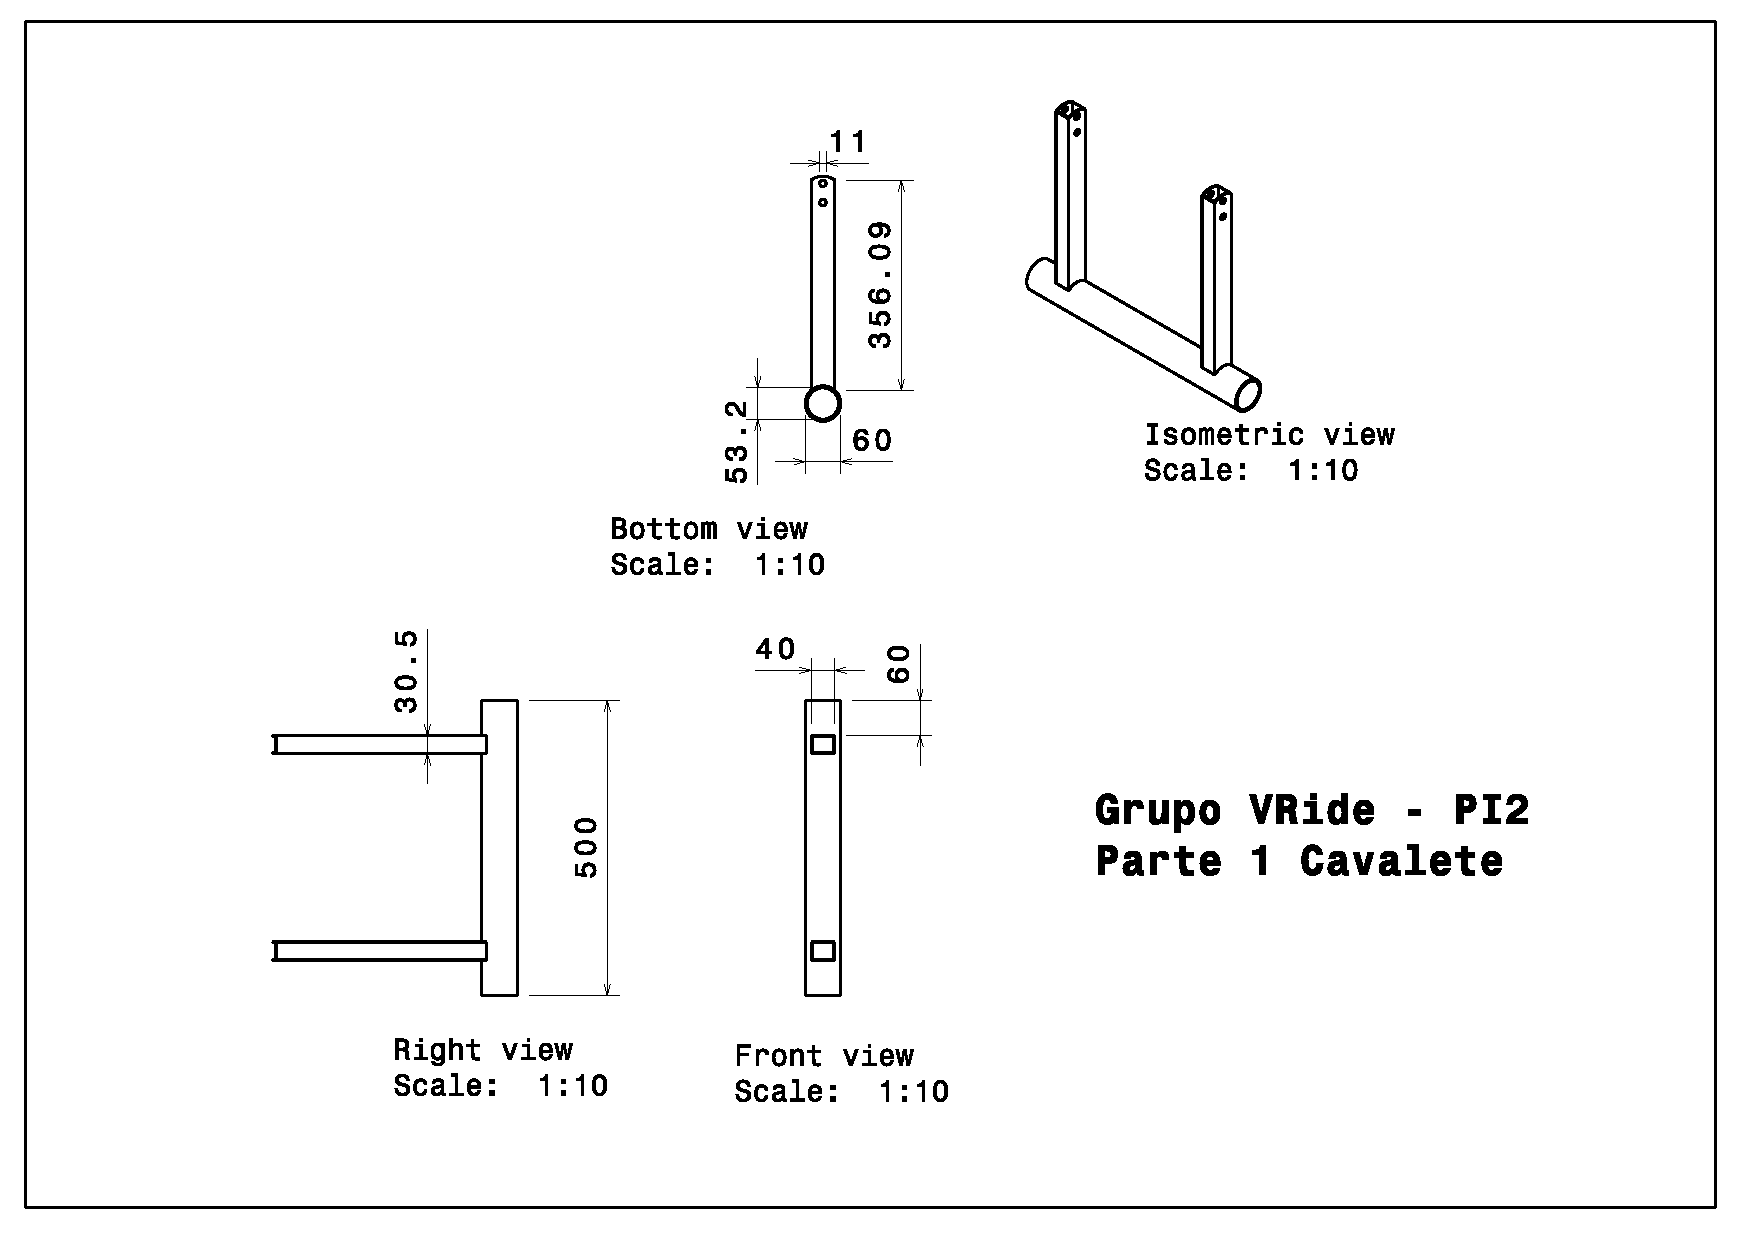
\includepdf[pages=1]{pdfs/dte_parte1_cavalete.pdf}  \label{anexo_pe_sem_rolo}
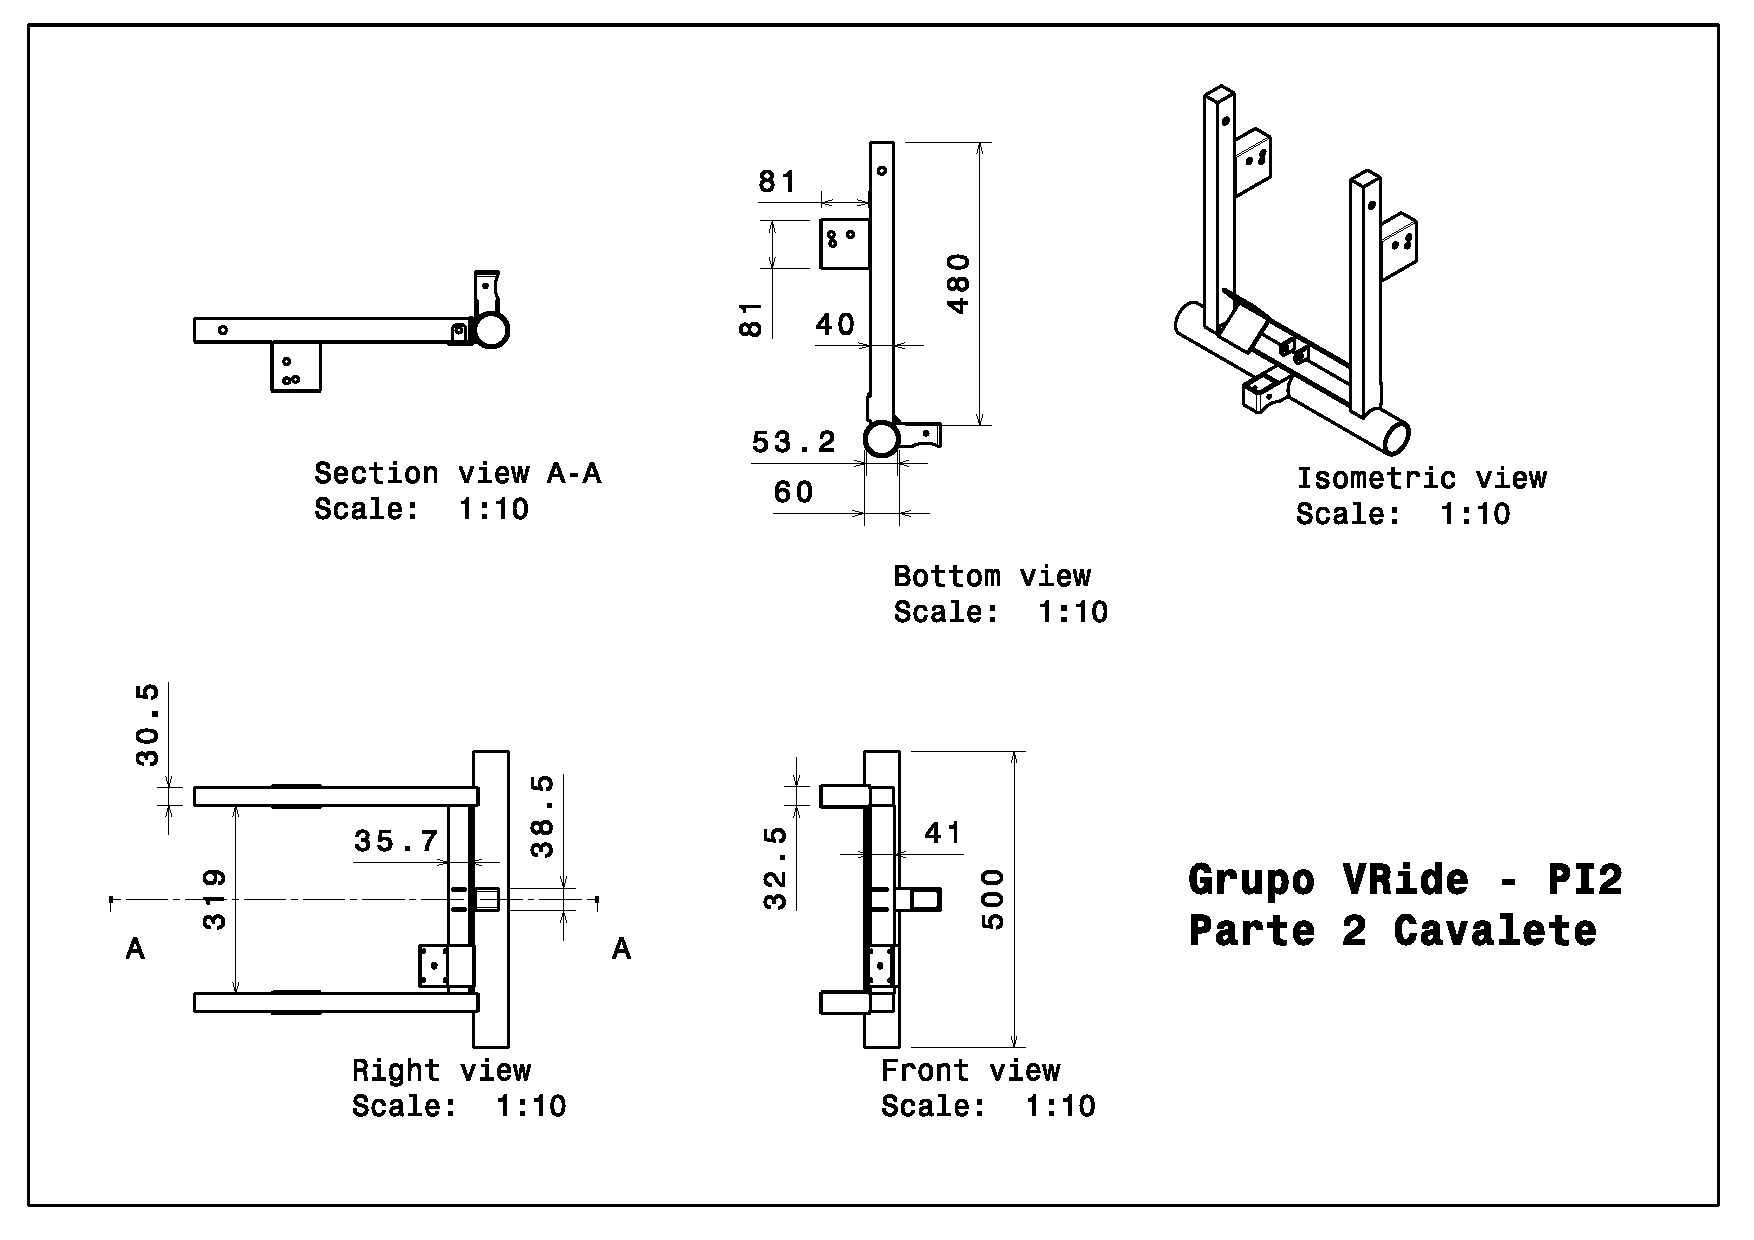
\includepdf[pages=1]{pdfs/dte_parte2_cavalete.pdf} \label{anexo_pe_com_rolo}
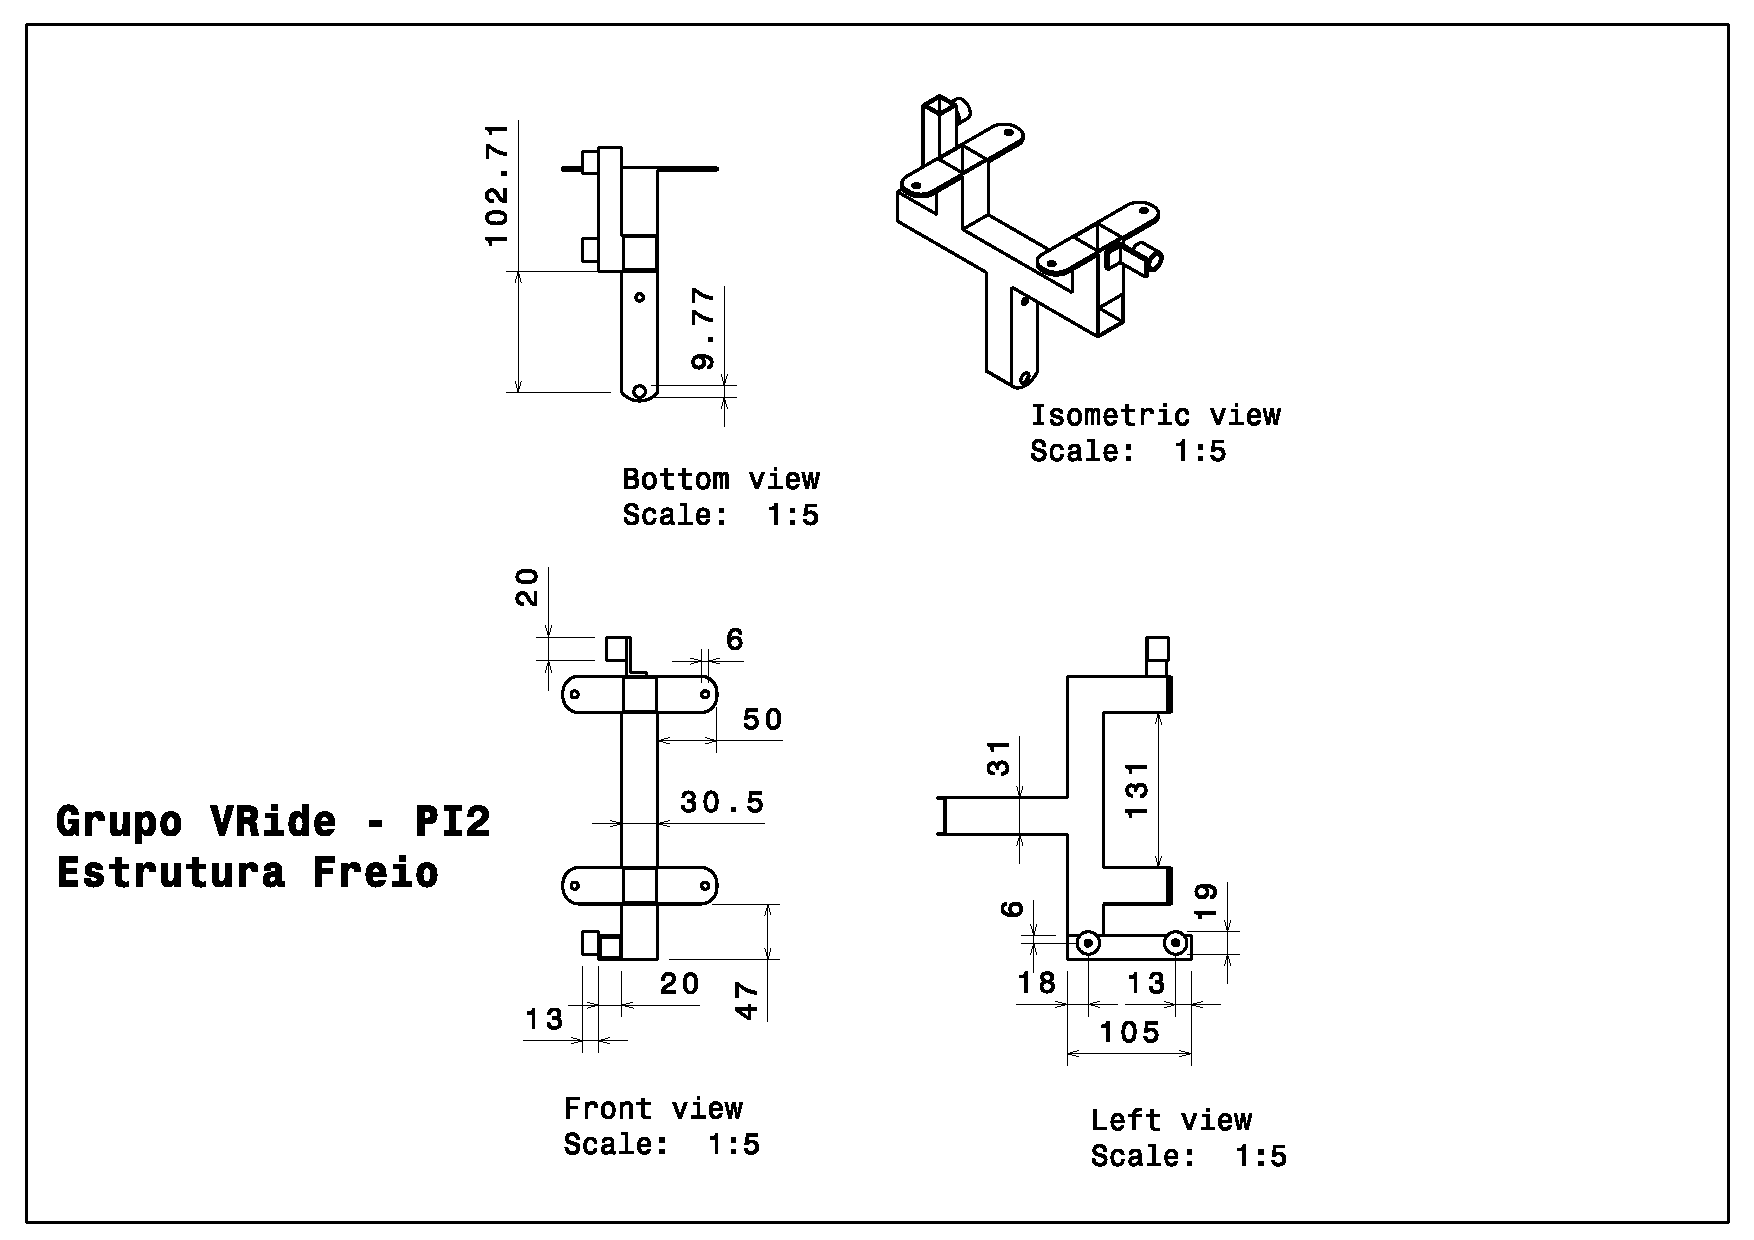
\includepdf[pages=1]{pdfs/dte_estrutura_freio.pdf} \label{anexo_estrutura_freio}
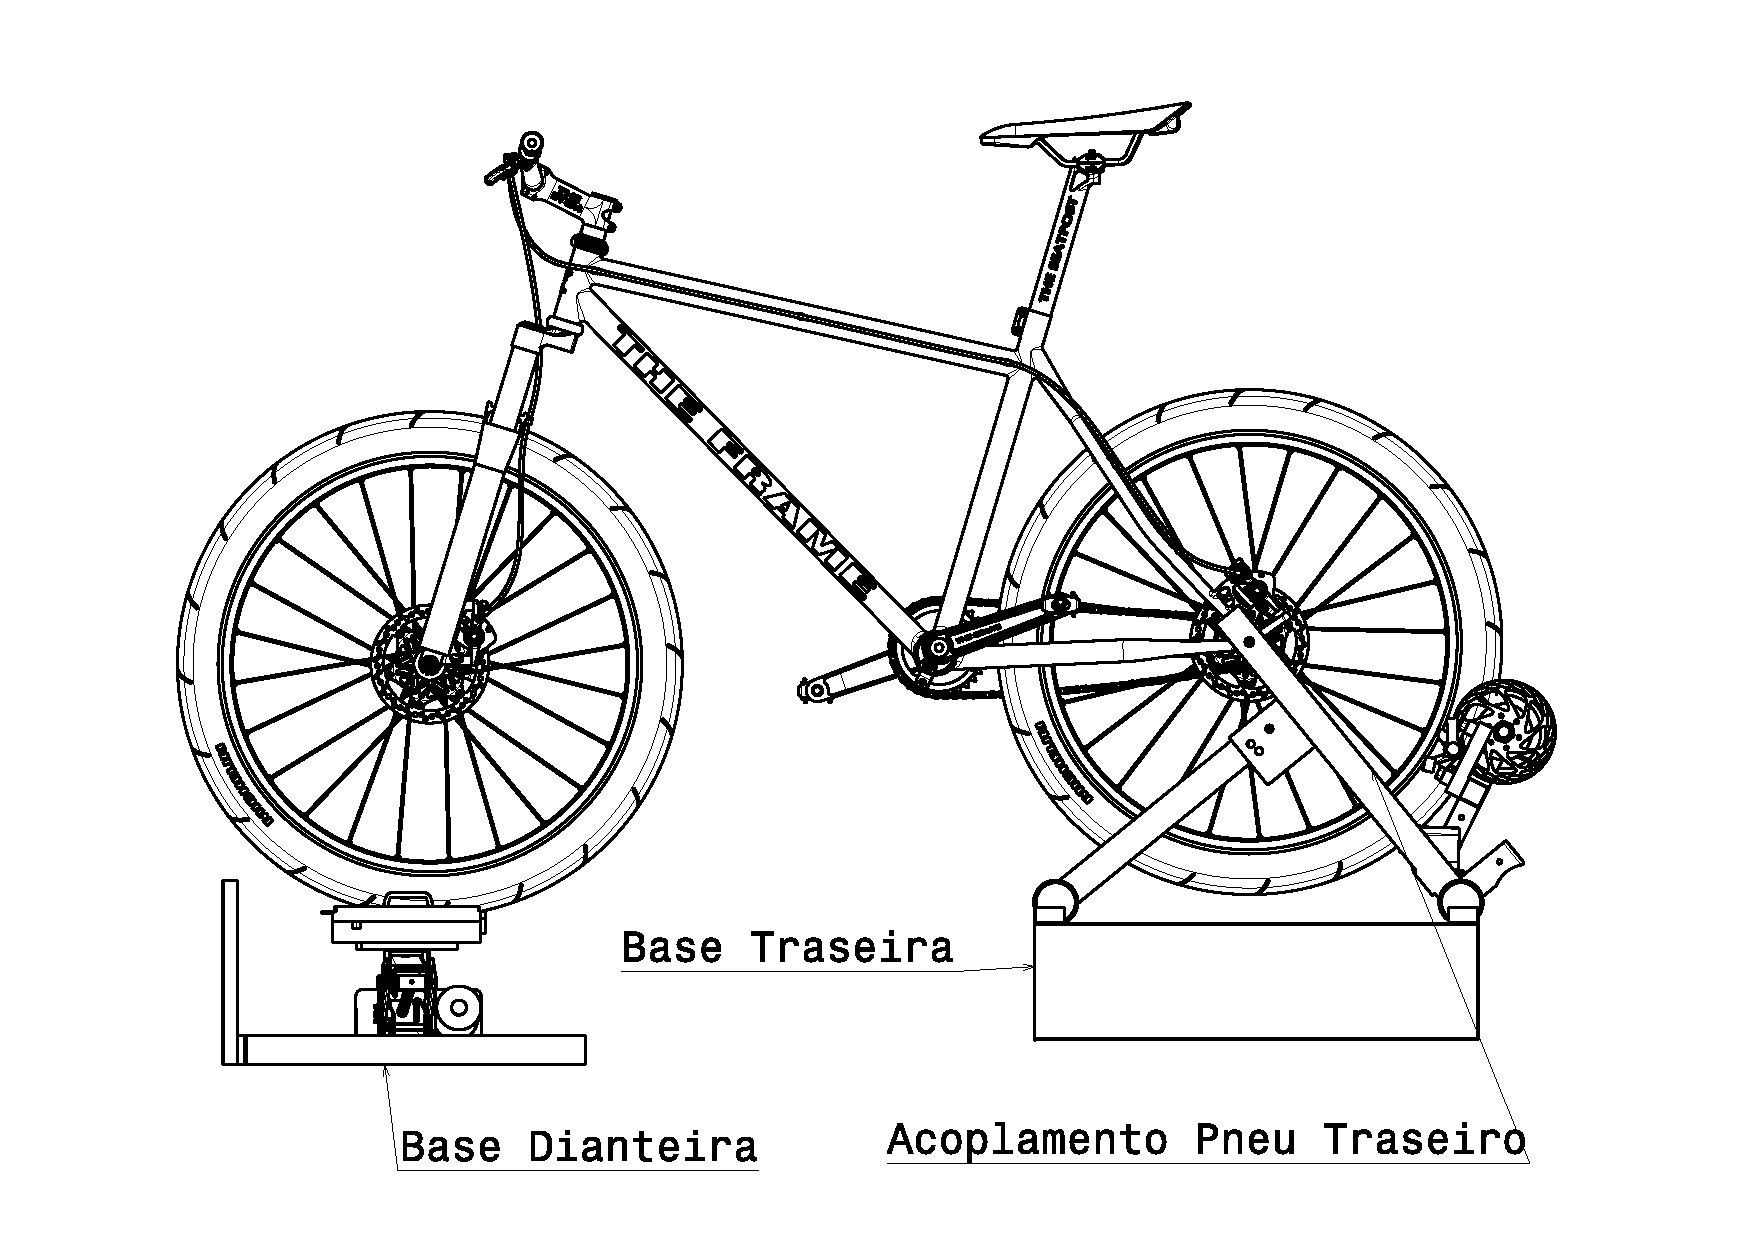
\includepdf[pages=1]{pdfs/dte_sistema_completo.pdf} \label{anexo_full}

\chapter{Análise de convergência de uma estrutura traseira de sustentação de bicicleta}
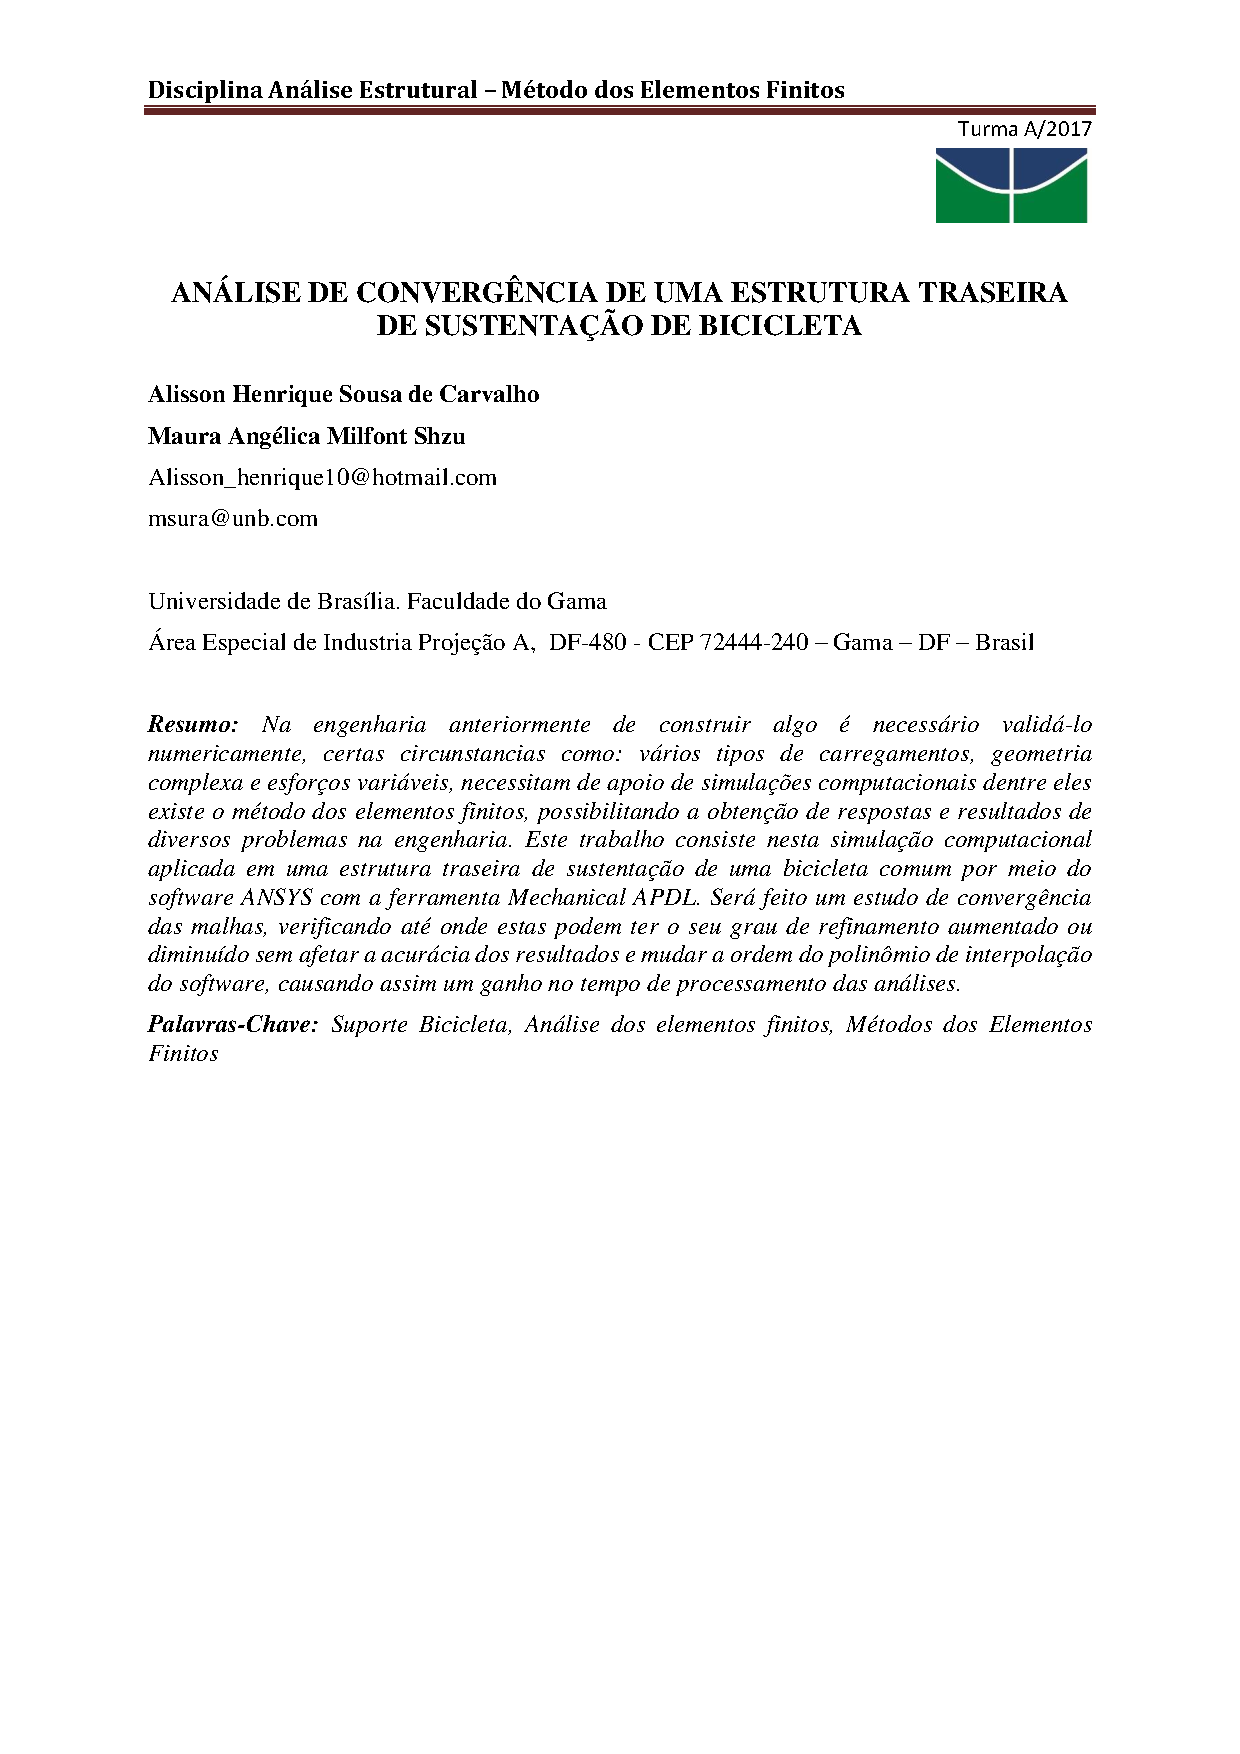
\includepdf[pages=1]{pdfs/RelatorioAlisson.pdf}

\chapter{Manual de Configuração}
O ambiente para desenvolver o jogo para o VRide é baseado nas versões da \textit{Unity} e do \textit{Oculus Integration}. Abaixo estão as versões de cada componente necessário para o ambiente funcionar no \textit{Oculus Development Kit} 1 (DK1):

\begin{itemize}
\item Unity3D 4.6.0
\item OVR Unity Integration 0.4.2lib
\item Oculus Runtime SDK 0.4.2
\end{itemize}

Com cada um destes itens baixados, segue a instalação passo a passo.

\section{Passo a passo}

Antes de prosseguir, verifique se você não possui nenhuma versão da \textit{Unity} instalada.

\begin{enumerate}
\item Instale a \textit{Unity} normalmente, clicando em próximo até terminar.

\item Para instalar o crack, siga estas etapas:

2.1. Copie o arquivo Unity.exe da pasta crack para a pasta \textit{Unity} (geralmente C: $\backslash$Program Files$\backslash$Unity$\backslash$Editor).

2.2. Copie o arquivo \textit{Unity\_v4.x.ulf} da pasta crack para dados \textit{Unity} (geralmente C: $\backslash$ProgramData$\backslash$Unity).

NOTA: Se esta pasta não aparecer, você precisa configurar para exibir as pastas ocultas.

\item Instale o \textit{Oculus Runtime}, \textit{oculus\_runtime\_rev\_1\_sdk\_0.4.2\_win.exe}, apenas pressionando seguir.

\item Extraia os arquivos de \textit{ovr\_unity\_0.4.2\_lib.zip}. Abra a \textit{Unity}, e então faça um duplo clique em \textit{OculusUnityIntegration.unitypackage}. Isso importará as coisas necessárias para executar o \textit{Oculus} na \textit{Unity}.

\item Para testar o \textit{Oculus}, é importante importar OculusUnityIntegrationTuscanyDemo.unitypackage. Na pasta Tuscany tem um projeto \textit{Unity}, quando clicar na barra lateral direita aparecerá um botão para abrir.

\item Antes de executar a demo, instale outros \textit{drivers} para executar o \textit{Oculus}. Eles estão em C: Usuário$\backslash$Seu nome de usuário$\backslash$AppData$\backslash$Local$\backslash$Temp$\backslash$Oculus Inc. Então, você precisa executar \textit{OculusDisplayDriver\_\Win8.1\_x64.msi} e \textit{OculusMSI\_x64.msi}.

\item Para testar que tudo está funcionando corretamente, execute o projeto em \textit{Unity}.
\end{enumerate}


\chapter{Manual de Empacotamento do Unity}
A seguir, está descrito os passos para gerar um pacote de um jogo no Unity.

\begin{enumerate}
\item Acessar Edit > Project Settings > Player.

\begin{center}
	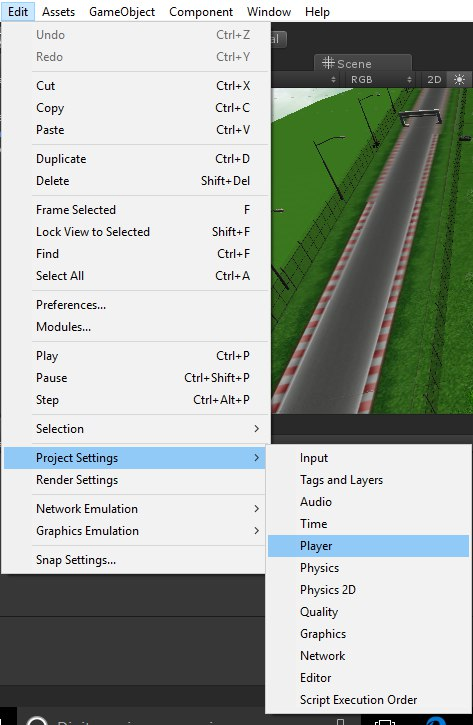
\includegraphics[scale=0.4]{figuras/playersettingspath}
	\captionof{figure}{Caminho para o Player Settings.}
\end{center}

\item Configurar as opções de configuração do Player como o nome do produto, o ícone, o nome da empresa, a resolução padrão do jogo, entre outras.

\begin{center}
	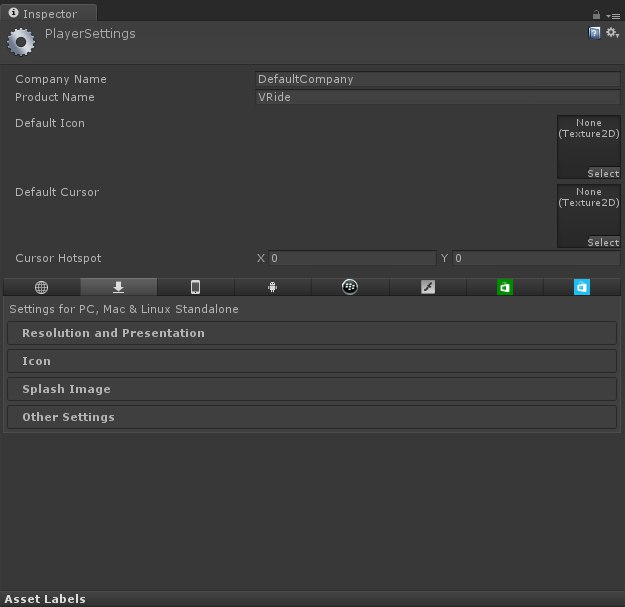
\includegraphics[scale=0.4]{figuras/playersettings}
	\captionof{figure}{Player Settings.}
\end{center}

\item Adicionar todas as cenas no Build Settings. Para isso, é necessário entrar na cena, acessar File > Build Settings e clicar em ``Add current''. As cenas devem ser ordenadas de acordo com o desejado para execução sendo 0 a primeira a ser executada.

\begin{center}
	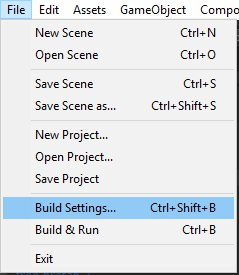
\includegraphics[scale=0.4]{figuras/buildsettingspath}
	\captionof{figure}{Caminho para o Build Settings.}
	\label{fig:buildsettings}
\end{center}

\begin{center}
	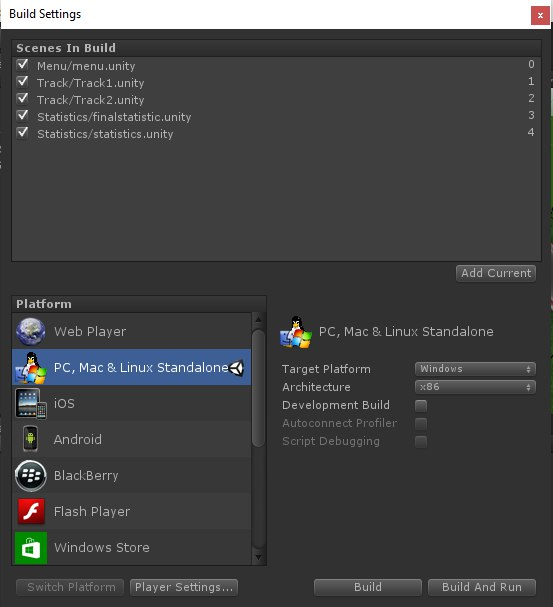
\includegraphics[scale=0.4]{figuras/buildsettings}
	\captionof{figure}{Build Settings.}
	\label{fig:buildsettings}
\end{center}

\item Ainda no Build Settings (Figura \ref{fig:buildsettings}), selecionar a plataforma desejada e apertar em Build.

\item Será carregado o pacote com a extensão desejada.
\end{enumerate}
  
\end{apendicesenv}
